
\documentclass{article}

\usepackage{etoolbox}


\usepackage{fullpage}
\usepackage{color}
\usepackage{amsmath}
\usepackage{url}
\usepackage{verbatim}
\usepackage{graphicx}
\usepackage{parskip}
\usepackage{amssymb}
\usepackage{float}
\usepackage{listings} % For displaying code

\begin{document}

\definecolor{blu}{rgb}{0,0,1}
\def\blu#1{{\color{blu}#1}}
\definecolor{gre}{rgb}{0,.5,0}
\def\gre#1{{\color{gre}#1}}
\definecolor{red}{rgb}{1,0,0}
\def\red#1{{\color{red}#1}}
\def\norm#1{\|#1\|}
\newcommand{\argmin}[1]{\mathop{\hbox{argmin}}_{#1}}
\newcommand{\argmax}[1]{\mathop{\hbox{argmax}}_{#1}}
\def\R{\mathbb{R}}
\newcommand{\fig}[2]{\includegraphics[width=#1\textwidth]{a3f/#2}}
\newcommand{\centerfig}[2]{\begin{center}\includegraphics[width=#1\textwidth]{a3f/#2}\end{center}}
\def\items#1{\begin{itemize}#1\end{itemize}}
\def\enum#1{\begin{enumerate}#1\end{enumerate}}
\def\argmax{\mathop{\rm arg\,max}}
\def\argmin{\mathop{\rm arg\,min}}
\def\half{\frac 1 2}
\newcommand{\code}[1]{\lstinputlisting[language=Matlab]{a3f/#1}}
\newcommand{\alignStar}[1]{\begin{align*}#1\end{align*}}
\newcommand{\mat}[1]{\begin{bmatrix}#1\end{bmatrix}}


%%%My commands
\newcommand{\p}{\mathbb{P}}
\newcommand{\x}{\textbf{x}}
\newcommand{\yy}{\tilde{y}^{i}}
\newcommand{\xx}{\tilde{x}^{i}}
\newcommand{\kk}{1-\sum_{c\neq (k,k)}\theta_{c}}



\title{CPSC 540 Assignment 3 (due February 27)}
\author{Juan Garcia}
\date{}
\maketitle


\section{Discrete and Gaussian Variables}

\subsection{MLE for General Discrete Distribution}

Consider a density estimation task, where we have two variables ($d=2$) that can each take one of $k$ discrete values. For example, we could have
\[
X = \mat{1 & 3\\4 & 2\\ $k$ & 3\\1 & $k-1$}.
\]
The likelihood for example $x^i$ under a general discrete distribution would be
\[
p(x^i_1, x^i_2 | \Theta) = \theta_{x_1^i,x_2^i},
\]
where $\theta_{c_1,c_2}$ gives the probability of $x_1$ being in state $c_1$ and $x_2$ being in state $c_2$, for all the $k^2$ combinations of the two variables. In order for this to define a valid probability, we need all elements $\theta_{c_1,c_2}$ to be non-negative and they must sum to one, $\sum_{c_1=1}^k\sum_{c_2=1}^k \theta_{c_1,c_2} = 1$.
\enum{
\item Given $n$ training examples, \blu{derive the MLE for the $k^2$ elements of $\Theta$}.
\item Because of the sum-to-1 constraint, there are only $(k^2 - 1)$ degrees of freedom in the discrete distribution, and not $k^2$. \blu{Derive the MLE for this distribution assuming that
\[
\theta_{k,k} = 1 - \sum_{c_1=1}^k\sum_{c_2=1}^{k}\mathcal{I}[c_1\neq k,c_2 \neq k]\theta_{c_1,c_2},
\]
}so that the distribution only has $(k^2-1)$ parameters.
\item If we had separate parameter $\theta_{c_1}$ and $\theta_{c_2}$ for each variables, a reasonable choice of a prior would be a product of Dirichlet distributions,
\[
p(\theta_{c_1},\theta_{c_2}) \propto \theta_{c_1}^{\alpha_{c_1} - 1}\theta_{c_2}^{\alpha_{c_2} - 1}.
\]
For the general discrete distribution, a prior encoding the same assumptions  would be
\[
p(\theta_{c_1,c_2}) \propto \theta_{c_1,c_2}^{\alpha_{c_1} + \alpha_{c_2} - 2}.
\]
\blu{Derive the MAP estimate under this prior}.
}
Hint: it is convenient to write the likelihood for an example $i$ in the form
\[
p(x^i | \Theta) = \prod_{c \in [k]^2}\theta_c^{\mathcal{I}[x^i = c]},
\]
where $c$ is a vector containing $(c_1,c_2)$, $[x^i = c]$ evaluates to 1 if all elements are equal, and $[k]^2$ is all ordered pairs $(c_1,c_2)$. You can use the Lagrangian to enforce the sum-to-1 constraint on the log-likelihood, and you may find it convenient to define $N_c = \sum_{i=1}^n \mathcal{I}[x^i = c]$.

\newpage
%%%%%%%%%%%%%%%%%%%%%%%%%%%%%%%%%%%%%%%%%%%%%%%%%%%%Exercise 1 %%%%%%%%%%%%%%%%%%%%%%%%%%%%%%%%%%%%%%%%%%%%%%%%%%%
\subsubsection*{Solution}
\textbf{1}. 
\newline
Having $n$ training examples $\textbf{x}:=(x^{1},\ldots,x^{n})$ where $x^{i}\in\{1,2,\ldots,k\}^{2}$ with
\begin{equation*}
\p(x_{1}^{i}=c_{1},x_{2}^{i}=c_{2})=\theta_{c1,c2}.
\end{equation*}
By denoting $\Theta$ the matrix containing all the parameters $\theta_{c_{1},c_{2}}$, we can write the likelihood for the $i$-th variable as
\begin{equation*}
\p(x^{i}|\Theta)=\prod_{c\in[k]^{2}}\theta_{c}^{\mathcal{I}[x^{i}=c]}.
\end{equation*}
By assuming independence between the variables we conclude 
\begin{eqnarray*}
\p(\x|\Theta)=\prod_{i=1}^{n}\p(x^{i}|\Theta)\\
=\prod_{i=1}^{n}\prod_{c\in[k]^{2}}\theta_{c}^{\mathcal{I}[x^{i}=c]}.
\end{eqnarray*}
Exchanging the order in the products and defining $N_c = \sum_{i=1}^n \mathcal{I}[x^i = c]$, we get
\begin{equation}\label{eqnmle}
\p(\x|\Theta)=\prod_{c\in[k]^{2}}\theta_{c}^{N_{c}}.
\end{equation}
Since the logarithm is an increasing function, the maximizer of this equation is the same as the maximizer of 
\begin{equation}\label{eqnloglikelihood}
\log(\p(\x|\Theta))=\sum_{c\in[k]^{2}}N_{c}\log(\theta_{c}).
\end{equation}
Since we want the parameters $\theta_{c}$ to represent probabilities, we have the constraint $\sum_{c\in [k]^{2}}\theta_{c}=1$. Hence
if we use Lagrange multipliers we conclude that for all $l\in [k]$ we have 
\begin{equation*}
\frac{\partial}{\partial\theta_{l}}(\log(\p(\x|\Theta)))=\lambda\frac{\partial}{\partial\theta_{l}}(\sum_{c\in [k]^{2}}\theta_{c}).
\end{equation*}
Derivating and solving for $\theta_{l}$ we conclude that
\begin{equation*}
\theta_{l}=\frac{N_{l}}{\lambda}.
\end{equation*}
Inserting this result into the constraint we get
\begin{equation*}
\lambda=\sum_{c\in [k]^{2}}N_c.
\end{equation*}
Hence the maximum likelihood estimation gives for each $l\in[k]^{2}$ 
\begin{equation*}
\theta_{l}=\frac{N_l}{\sum_{c\in[k]^{2}}N_c}.
\end{equation*}
\newpage

\textbf{2}.
\newline
In this case by assuming $\theta_{k,k}=1-\sum_{c\neq (k,k)}\theta_{c}$ we modify equation (\ref{eqnmle}) to get
\begin{equation*}
\p(\x|\Theta)=(\kk)^{\alpha}\prod_{c\neq (k,k)}\theta_{c}^{N_{c}},
\end{equation*}
where $\alpha=n-\sum_{c\neq (k,k)}N_{c}$. By taking $\log$ on both sides of the equation, we obtain
\begin{equation*}
\log(\p(\x|\Theta))=\alpha\log(\kk)+\sum_{c\neq (k,k)}N_{c}\log(\theta_{c}).
\end{equation*}
By letting $c=(c1,c2)$ and taking the derivative with respect to $\theta_{mn}$ we get
\begin{equation*}
\frac{\partial}{\partial\theta_{mn}}(\log(\p(\x|\Theta)))=\frac{-\alpha\delta_{(m,n)(c_{1},c_{2})}\theta_{c_{1},c_{2}}}{1-\sum_{(c_{1},c_{2})\neq (k,k)}\theta_{c_1,c_2}}
+\sum_{(c_{1},c_{2})\neq (k,k)}\frac{N_{c}}{\theta_{c_{1},c_{2}}}\delta_{(m,n)(c_{1},c_{2})}.
\end{equation*}
Simplifying and equating to zero we obtain
\begin{equation*}
\frac{\alpha\theta_{m,n}}{\kk}-\frac{N_{m,n}}{\theta_{m,n}}=0.
\end{equation*}
If we define $A_{mn}=\sum_{c\neq (k,k),c\neq (m,n)}$ then we get
\begin{equation*}
\alpha\theta_{mn}^{2}+N_{mn}\theta_{mn}+N_{mn}(A_{mn}-1)=0.
\end{equation*}
With this we have $n\times m$ equations to solve for the $n\times m$ parameters. The solution gives us the vales of $\Theta$ for the MLE. Clearly is easier to use Lagrange Multipliers.
\newpage


\textbf{3}. 
\newline
We want to find the MAP for $\p(\Theta|\x)$ or $\log(\p(\Theta|\x))$. Using Bayes rule we get
\begin{equation*}
\p(\Theta|\x)\propto\p(\x|\Theta)\p(\Theta).
\end{equation*}
Choosing the prior 
\begin{equation*}
\p(\Theta)=\prod_{(c_{1},c_{2})\in [k]^{2}}\theta_{c1,c2}^{\alpha_{c_{1}}+\alpha_{c_{2}}-2}.
\end{equation*}
We can easily see that 
\begin{equation*}
\log(\p(\Theta))=\sum_{(c_1,c_2)\in [k]^{2}}(\alpha_{c_{1}}+\alpha_{c_{2}}-2)\log(\theta_{c_1,c_2}).
\end{equation*}
Combining this result with equation (\ref{eqnloglikelihood}) we get that the log posterior is given by
\begin{equation*}
\log(\p(\Theta|\x))=\underbrace{\sum_{(c_1,c_2)\in[k]^{2}}N_{c_1,c_2}\log(\theta_{c_1,c_2})}_{\log(\p(\x|\Theta))}+
\underbrace{\sum_{(c_1,c_2)\in [k]^{2}}(\alpha_{c_{1}}+\alpha_{c_{2}}-2)\log(\theta_{c_1,c_2})}_{\log(\p(\Theta))}.
\end{equation*}
Using the sum to one constraint and Lagrange multipliers we conclude that for all $(l_{1},l_{2})\in [k]^{2}$ we must  have
\begin{equation*}
\frac{\partial}{\partial\theta_{l_1,l_2}}(\sum_{(c_1,c_2)\in[k]^{2}}N_{c_1,c_2}\log(\theta_{c_1,c_2})+
\sum_{(c_1,c_2)\in [k]^{2}}(\alpha_{c_{1}}+\alpha_{c_{2}}-2)\log(\theta_{c_1,c_2}))=
\lambda\frac{\partial}{\partial\theta_{l_1,l_2}}(\sum_{(c_1,c_2)\in [k]^{2}}\theta_{c_1,c_2})
\end{equation*}
Taking the derivatives and solving for $\theta_{l_1,l_2}$ we get
\begin{equation*}
\theta_{l1,l2}=\frac{N_{l1,l2} +\alpha_{l_{1}}+\alpha_{l_{2}}-2}{\lambda}.
\end{equation*}
Plugging in this value into the sum to one constraint we conclude
\begin{equation*}
\lambda=\sum_{(c_1,c_2)\in [k]^{2}}N_{c1,c2}+\alpha_{c_{1}}+\alpha_{c_{2}}-2.
\end{equation*}
Hence the MAP estimate is


\begin{equation*}
\theta_{l1,l2}=\frac{N_{l1,l2} +\alpha_{l_{1}}+\alpha_{l_{2}}-2}{\sum_{(c_1,c_2)\in [k]^{2}}N_{c1,c2}+\alpha_{c_{1}}+\alpha_{c_{2}}-2}.
\end{equation*}

\newpage
\subsection{Generative Classifiers with Gaussian Assumption}

Consider the 3-class classification dataset in this image:
%\centerfig{.4}{sample}
In this dataset, we have 2 features and each colour represents one of the classes. Note that the classes are highly-structured: the colours each roughly follow a Gausian distribution plus some noisy samples.

Since we have an idea of what the features look like for each class, we might consider classifying  inputs $x$ using a \emph{generative classifier}. In particular, we are going to use Bayes rule to write
\[
p(y=c|x,\Theta) = \frac{p(x| y=c, \Theta) \cdot p(y=c|\Theta)}{p(x|\Theta)},
\]
where $\Theta$ represents the parameters of our model. To classify a new example $\hat{x}$, generative classifiers would use
\[
\hat{y} = \argmax_{y \in \{1,2,\dots,k\}} p(\hat{x}| y=c,\Theta)p(y=c|\Theta),
\]
where in our case the total number of classes $k$ is $3$ (The denominator $p(\hat{x}|\Theta)$ is irrelevant to the classification since it is the same for all $y$.)
% and $\theta_c$ is the set of parameters associated class $c$.
Modeling $p(y=c|\Theta)$ is eays: we can just use a $k$-state categorical distribution,
\[
p(y = c | \Theta) = \theta_c,
\]
where $\theta_c$ is a single parameter for class $c$. The maximum likelihood estimate of $\theta_c$ is given by $n_c/n$, the number of times we have $y^i = c$ (which we've called $n_c$) divided by the total number of data points $n$.

Modeling $p(x | y =c, \Theta)$ is the hard part: we need to know the \emph{probability of seeing the feature vector $x$ given that we are in class $c$}. This corresponds to solving a density estimation problem for each of the $k$ possible classes. 
To make the density estimation problem tractable, we'll assume that the distribution of $x$ given that $y=c$ is given by a $\mathcal{N}(\mu_c,\Sigma_c)$ Gaussian distribution for a class-specific $\mu_c$ and $\Sigma_c$,
\[
p(x | y=c, \Theta) = \frac{1}{(2\pi)^{\frac{d}{2}}|\Sigma_c|^{\half}}\exp\left(-\half (x-\mu_c)^T\Sigma_c^{-1}(x-\mu_c)\right).
\]
Since we are distinguishing between the probability under $k$ different Gaussians to make our classification, this is called \emph{Gaussian discriminant analysis} (GDA). In the special case where we have a constant $\Sigma_c = \Sigma$ across all classes it is known as \emph{linear discriminant analysis} (LDA) since it leads to a linear classifier between any two classes (while the region of space assigned to each class forms a convex polyhedron as in $k$-means clustering). Another common restriction on the $\Sigma_c$ is that they are diagonal matrices, since this only requires $O(d)$ parameters instead of $O(d^2)$ (corresponding to assuming that the features are independent univariate Gaussians given the class label).
Given a dataset $\mathcal{D}=\{(x^i, y^i)\}_{i=1}^n$, where $x^i\in\R^d$ and $y^i\in\{1,\ldots,k\}$, the maximum likelihood estimate (MLE) for the $\mu_c$ and $\Sigma_c$ in the GDA model is the solution to
\[
\argmax_{\mu_1,\mu_2,\dots,\mu_k,\Sigma_1,\Sigma_2,\dots,\Sigma_k} \prod_{i=1}^n p(x^i | y^i, \mu_{y^i},\Sigma_{y^i}).
\]
This means that the negative log-likelihood will be  equal to
\alignStar{
- \log p(X|y,\Theta) & = -\sum_{i=1}^n \log p(x^i | y^i | \mu_{y^i},\Sigma_{y^i})\\
& = \sum_{i=1}^n \frac{1}{2}(x^i - \mu_{y^i})^T\Sigma_{y^i}^{-1}(x^i - \mu_{y^i}) + \half\sum_{i=1}^n \log|\Sigma_{y^i}| + \text{const.}
}

\enum{
\item \blu{Derive the MLE for the GDA model under the assumption of \emph{common diagonal covariance} matrices}, $\Sigma_c = D$ ($d$ parameters). (Each class will have its own mean $\mu_c$.)
\item \blu{Derive the MLE for the GDA model under the assumption of \emph{individual scale-identity} matrices}, $\Sigma_c = \sigma_c^2 I$ ($k$ parameters).
\item It's painful to derive these from scratch, but you should be able to see a pattern that would allow other common restrictions. Without deriving the result from scratch (hopefully), \blu{give the MLE for the case of \emph{individual full} covariance matrices}, $\Sigma_c$ ($O(kd^2)$ parameters).
\item When you run \emph{example\_generative} it loads a variant of the dataset in the figure that has 12 features and 10 classes. This data has been split up into a training and test set, and the code fits a $k$-nearest neighbour classifier to the training set then reports the accuracy on the test data ($\sim 36\%$). The $k$-nearest neighbour model does poorly here since it doesn't take into account the Gaussian-like structure in feature space for each class label. Write a function \emph{generativeGaussian} that fits a GDA model to this dataset (using individual full covariance matrices). \blu{Hand in the function and report the test set accuracy}.
\item In this question we would like to replace the Gaussian distribution of the previous problem with the more robust multivariate-t distribution so that it isn't influenced as much by the noisy data.
Unlike the previous case, we don't have a closed-form solution for the parameters. However, if you run \emph{example\_tdist} it generates random noisy data and fits a multivariate-t model (you will need to add the \emph{minFunc} directory to the Matlab path for the demo to work). By using the \emph{multivariateT} model, write a new function \emph{generativeStudent} that implements a generative model that is based on the multivariate-t distribution instead of the Gaussian distribution. \blu{Report the test accuracy  with this model.}
}
Hints: you will be able to substantially simplify the notation in parts 1-3 if you use the notation $\sum_{i \in y_c}$ to mean the sum over all values $i$ where $y^i = c$. Similarly, you can use $n_c$ to denote the number of cases where $y_i = c$, so that we have $\sum_{i \in y_c}1 = n_c$. Note that the determinant of a diagonal matrix is the product of the diagonal entries, and the inverse of a diagonal matrix is a diagonal matrix with the reciprocals of the original matrix along the diagonal. For part three you can use the result from class regarding the MLE of a general multivariate Gaussian. You may find it helpful to use the included \emph{logdet.m} function to compute the log-determinant in more numerically-stable way.

%%%%%%%%%%%%%%%%%%%%%%%%%%%%%%%%%%%%%%%%%%%%%%%%Exercise 2 %%%%%%%%%%%%%%%%%%%%%%%%%%%%%%%%%%%%%%%%%%%%%%%%%%%%%%%%%
\newpage
\subsubsection*{Solution}
\textbf{1}. 
\newline
Under the assumption that $\Sigma_{c}=D$ where $D$ diagonal, the negative log-likelihood becomes
\begin{equation*}
- \log \p(X|y,\Theta)
 = \sum_{i=1}^n \frac{1}{2}(x^i - \mu_{y^i})^TD^{-1}(x^i - \mu_{y^i}) + \half\sum_{i=1}^n \log|D| + \text{const.}
\end{equation*}
This is a quadratic function in the $\mu_{y^{i}}$ variables, hence it has a unique minimum. By taking the gradient with respect to $\mu_{c}$ 
and equating it to zero we get
\begin{equation*}
\nabla_{\mu_{c}}(-log(\p(X|y,\theta)))=\sum_{i\in y_{c}}D^{-1}(\mu_{c}-x^{i})=0,
\end{equation*}
in this last equation we used the identity $\nabla_{z} (z^{T}Az)=(A+A^{T})z$, and the fact that $D^{-1}$ is symmetric.
Solving for $\mu_{c}$ we get
\begin{equation*}
\mu_{c}\sum_{i\in y_{c}}1=D\sum_{i\in y_{c}}D^{-1}x^{i}.
\end{equation*}
If we denote $N_{c}=\sum_{i\in y_{c}}1$ and multiply $D$ with $D^{-1}$  we conclude that
\begin{equation*}
\mu_{c}=\frac{1}{N_{c}}\sum_{i\in y_{c}}x^{i}.
\end{equation*}
That is, the maximum likelihood estimate for the mean is the the average over all features that correspond to the class $c$.

To calculate the MLE estimate for $D$, let us assume that $D=diag(\frac{1}{\lambda_{1}},\ldots,\frac{1}{\lambda_{d}})$, hence
$D^{-1}=diag(\lambda_{1},\ldots,\lambda_{d})$. Hence we have
\begin{equation*}
- \log \p(X|y,\Theta)=\sum_{i=1}^{n} \frac{1}{2}\sum_{j=1}^{d}\lambda_{j}(x^{i}-\mu_{y^{i}})^{2}_{j}+\frac{1}{2}\sum_{i=1}^{n}\log(\prod_{j=1}^{d}\frac{1}{\lambda_{j}})+const.
\end{equation*}
In this equation the subscript $j$ in $(x^{i}-\mu_{y^{i}})_{j}$ means the $j$-th component of the vector. Using the properties of the logarithm we get

\begin{equation*}
- \log \p(X|y,\Theta)=\frac{1}{2}\sum_{i=1}^{n}\sum_{j=1}^{d}\lambda_{j}(x^{i}-\mu_{y^{i}})^{2}_{j}-\frac{1}{2}\sum_{i=1}^{n}\sum_{j=1}^{d}\log(\lambda_{j})+const.
\end{equation*}
Taking the partial derivative with respect to the $l$-th element and equating to $0$ we get
\begin{equation*}
\frac{\partial}{\partial\lambda_{l}}(- \log \p(X|y,\Theta))=\frac{1}{2}\sum_{i=1}^{n}(x^{i}-\mu_{y^{i}})^{2}_{l}-\frac{n}{2}\frac{1}{\lambda_{l}}=0.
\end{equation*}
Solving for $\lambda_{l}$ we conclude
\begin{equation*}
\lambda_{l}=\frac{1}{n}\sum_{i=1}^{n}(x^{i}-\mu_{y^{i}})^{2}_{l}.
\end{equation*}
This means that the best estimate for the $l$-th element in the diagonal of $D^{-1}$ is the estimate of the variance along the $l$-th coordinate direction.
\newpage

\textbf{2}. 
\newline
Now we are going to assume that $\Sigma_{c}=\sigma_{c}I$. With this assumption the negative log-likelihood becomes
\begin{equation*}
- \log \p(X|y,\Theta)
 = \sum_{i=1}^n \frac{1}{2\sigma_{y^{i}}^{2}}\underbrace{(x^i - \mu_{y^i})^T(x^i - \mu_{y^i})}_{\|x^{i}-\mu_{y^{i}}\|^{2}_{2}} + \half\sum_{i=1}^n \log|\sigma_{y^{i}}^{2}I| + \text{const.}
\end{equation*}
Again this is a quadratic function in terms of the means, hence by finding the gradient and equating to zero we find the unique minimizer. For the $c$ class label we have
\begin{equation*}
\nabla_{\mu_{c}}(-log(\p(X|y,\theta)))=\sum_{i\in y_{c}}\frac{1}{\sigma_{c}^{2}}(\mu_{c}-x^{i})=0.
\end{equation*}
Solving for the mean we get
\begin{equation}\label{eqnmus}
\mu_{c}=\frac{1}{N_{c}}\sum_{i\in y_{c}}x^{i}.
\end{equation}
Now we are going to find the MLE for the $\sigma_{c}$. To do so we find the partial derivative with respect to $\sigma_{l}$ of the negative log-likelihood to get
\begin{equation*}
\frac{\partial }{\partial\sigma_{l}}(- \log \p(X|y,\Theta))=-\frac{1}{\sigma_{l}^{3}}\|x^{l}-\mu_{l}\|^{2}+\frac{d}{\sigma_{l}}=0.
\end{equation*}
Solving for $\sigma^{2}$ we conclude
\begin{equation}\label{eqnsigmas}
\sigma_{l}^{2}=\frac{\|x^{l}-\mu_{l}\|^{2}}{d}.
\end{equation}
This is the MLE estimate for the variances.
\newpage
\textbf{3}. 
\newline
Finally for the general case, the likelihood is 
\begin{equation*}
-\log(\p(X|y,\Theta) = \sum_{i=1}^n \frac{1}{2}(x^i - \mu_{y^i})^T\Sigma_{y^i}^{-1}(x^i - \mu_{y^i}) + \half\sum_{i=1}^n \log|\Sigma_{y^i}| + \text{const.}
\end{equation*}
Again, taking the derivative with respect to $\mu_{c}$ and equate to $0$  we get
\begin{equation*}
\nabla_{\mu_{c}}(-\log(\p(X|y,\Theta))=\sum_{i\in y_{c}}\Sigma_{c}^{-1}(\mu_{c}-x^{i})=0.
\end{equation*}

Solving for $\mu_{c}$ we get the same result as in the two previous cases, namely 
\begin{equation*}
\mu_{c}=\frac{1}{N_{c}}\sum_{i\in y_{c}}x^{i}.
\end{equation*}
For the covariance, things are a little bit more tricky. First recall that given a matrix $A$ we have
\begin{equation}\label{eqnlogtraceidentity}
\nabla_{A}\log|A|=A^{-T}.
\end{equation}
On the other hand we have for matrices $A$ and $B$
\begin{equation*}
\nabla_{A}tr(BA)=B^{T}.
\end{equation*}
Since for any $c$ we have that $(x^{i}-\mu_{c})^{T}\Sigma_{c}^{-1}(x^{i}-\mu_{c})$ is a number then
\begin{equation*}
tr((x^{i}-\mu_{c})^{T}\Sigma_{c}^{-1}(x^{i}-\mu_{c}))=tr((x^{i}-\mu_{c})(x^{i}-\mu_{c})^{T}\Sigma_{c}^{-1}).
\end{equation*}
Hence
\begin{equation*}
\nabla_{\Sigma_{c}^{-1}}(tr((x^{i}-\mu_{c})(x^{i}-\mu_{c})^{T}\sigma_{c}^{-1}))=(x^{i}-\mu_{c})(x^{i}-\mu_{c})^{T}.
\end{equation*}
Combining this result with equation (\ref{eqnlogtraceidentity}) we conclude
\begin{equation*}
\frac{\partial}{\partial\Sigma_{c}}(-\log(\p(X|y,\Theta)))=\frac{1}{2}\sum_{i\in y_{c}}(x^{i}-\mu_{c})(x^{i}-\mu_{c})^{T}-\frac{N_{c}}{2}\Sigma_{c},
\end{equation*}
where in the last term we use the symmetry of $\Sigma_{c}$. Equating to $0$ and solving for $\Sigma_{c}$ we conclude
\begin{equation*}
\Sigma_{c}=\frac{1}{N_{c}}\sum_{i\in y_{c}}(x^{i}-\mu_{c})(x^{i}-\mu_{c})^{T}.
\end{equation*}
This gives the MLE for the covariance matrix of the $c$ class.
\newline

\textbf{4}.
\newline
Using the script generativeGaussian.m and running the script example$\_$Generative.m we get the following output
\begin{verbatim}
>> example_generative
Gaussian Gen. Model. accuracy is 0.63
\end{verbatim}
That is, we have an accuracy of $63\%$ in the test set.
\newline
\textbf{5}.
\newline
Using the script generativeStudent.m and running the script example$\_$Generative.m we get the following output
\begin{verbatim}
>> example_generative
Gaussian Gen. Model. accuracy is 0.63
Fitting multivariate student T density model...
Fitting multivariate student T density model...
Fitting multivariate student T density model...
Fitting multivariate student T density model...
Fitting multivariate student T density model...
Fitting multivariate student T density model...
Fitting multivariate student T density model...
Fitting multivariate student T density model...
Fitting multivariate student T density model...
Fitting multivariate student T density model...
Tdist Gen. Model. accuracy is 0.79
\end{verbatim}
In this case the accuracy is improved and we get $79\%$ of accuracy.


\newpage
\subsection{Self-Conjugacy for the Mean Parameter}

If $x$ is distributed according to a Gaussian with mean $\mu$,
\[
x \sim \mathcal{N}(\mu,\sigma^2),
\]
and we assume that $\mu$ itself is distributed according to a Gaussian
\[
\mu \sim \mathcal{N}(\alpha,\gamma^2),
\]
then the posterior $\mu | x$ also follows a Gaussian distribution.\footnote{We say that the Gaussian distribution is the `conjugate prior' for the Gaussian mean parameter (we'll formally discuss conjugate priors later in the course). Another reason the Gaussian distribution is important is that is the only (non-trivial) continuous distribution that has this `self-conjugacy' property.} \blu{Derive the form of the (Gaussian) distribution for $p(\mu|x,\alpha,\sigma^2,\gamma^2)$.} %You can assume that $\sigma=1$ and $\gamma=1$.

Hints: Use Bayes rule and use the $\propto$ sign to get rid of factors that don't depend on $\mu$. You can ``complete the square'' to make the product look like a Gaussian distribution, e.g. when you have $\exp(ax^2 - bx + \text{const})$ you can factor out an $a$ and add/subtract $(b/2a)^2$ to re-write it as
\begin{align*}
\exp\left(ax^2 - bx + const\right) & \propto
\exp\left(ax^2 - bx\right) = \exp\left(a(x^2 - (b/a)x)\right) \\& \propto \exp\left(a(x^2 - (b/a)x + (b/2a)^2)\right) =  \exp\left(a(x - (b/2a))^2\right).
\end{align*}
Note that multiplying by factors that do not depend on $\mu$ within the exponent does not change the distribution. In this question you will want to complete the square to get the distribution on $\mu$, rather than $x$.
You may find it easier to solve thie problem if you parameterize the Gaussians in terms of their `precision' parameters (e.g., $\lambda = 1/\sigma^2$, $\lambda_0 = 1/\gamma^2$) rather than their variances $\sigma^2$ and $\gamma^2$.

\newpage
\subsubsection*{Solution}
By Bayes rule the posterior can be computed as
\begin{equation*}
\p(\mu|x,\alpha,\sigma^2,\gamma^2)\propto\p(x|\mu,\alpha,\sigma^{2},\gamma^{2})\p(\mu|\alpha,\gamma^{2}).
\end{equation*}
By normality hypothesis on the likelihood and the prior we may write
\begin{equation*}
\p(\mu|x,\alpha,\sigma^2,\gamma^2)\propto\exp(-\frac{\lambda}{2}(x-\mu)^{2})\exp(-\frac{\lambda_{0}}{2}(\mu-\alpha)^{2}),
\end{equation*}
where $\lambda=\frac{1}{\sigma^{2}}$ and $\lambda_{0}=\frac{1}{\gamma^{2}}$. Combining the exponentials we get
\begin{equation*}
\p(\mu|x,\alpha,\sigma^2,\gamma^2)\propto \exp(-\frac{1}{2}(\lambda(x-\mu)^{2}+\lambda_{0}(\mu-\alpha)^{2})).
\end{equation*}
Expaning squares and keeping only terms depending on $\mu$ we obtain
\begin{equation*}
\p(\mu|x,\alpha,\sigma^2,\gamma^2)\propto\exp(-\frac{1}{2}(\lambda\mu^{2}-2\mu\lambda x+\lambda_{0}\mu^{2}-2\mu\lambda_{0}\alpha)).
\end{equation*}
Rearranging this equation can be cast into
\begin{equation*}
\p(\mu|x,\alpha,\sigma^2,\gamma^2)\propto\exp(-\frac{1}{2}((\lambda+\lambda_{0})\mu^{2}-2\mu(\lambda x+\lambda_{0}\alpha))).
\end{equation*}
To complete squares we need to add and substract the term $\left(\frac{\lambda x+\lambda_{0}\alpha}{\lambda+\lambda_{0}}\right)^{2}$. Since adding this term
is equivalent to add a constant term with respect to $\mu$ we may complete squares by just writing 
\begin{equation*}
\p(\mu|x,\alpha,\sigma^2,\gamma^2)\propto\exp(-\frac{1}{2}((\lambda+\lambda_{0})\mu^{2}-2\mu(\lambda x+\lambda_{0}\alpha)+\left(\frac{\lambda x+\lambda_{0}\alpha}{\lambda+\lambda_{0}}\right)^{2})).
\end{equation*}
Factoring the argument in the expoonential we get
\begin{equation*}
\p(\mu|x,\alpha,\sigma^2,\gamma^2)\propto\exp(-\frac{1}{2}\left(\sqrt{\lambda+\lambda_{0}}\mu-\frac{\lambda x+\lambda_{0}\alpha}{\lambda+\lambda_{0}}\right)^{2}).
\end{equation*}
Factoring the term to the left of $\mu$, this equation is written as
\begin{equation*}
\p(\mu|x,\alpha,\sigma^2,\gamma^2)\propto\exp(-\frac{\lambda+\lambda_{0}}{2}\left(\mu-\frac{\lambda x+\lambda_{0}\alpha}{(\lambda+\lambda_{0})^{\frac{3}{2}}}\right)^{2}).
\end{equation*}
This says that $\mu$ has also Gaussian distribution. More explicitly
\begin{equation*}
\mu|x,\alpha,\sigma^2,\gamma^2\sim\mathcal{N}(\frac{\lambda x+\lambda_{0}\alpha}{(\lambda+\lambda_{0})^{\frac{3}{2}}},\frac{1}{\lambda+\lambda_{0}}).
\end{equation*}
\newpage





%%%%%%%%%%%%%%%%%%%%%%%%%%%%%%%%%%%%%%%%%%%%%%%%%%%%%%%%%%%%%%%%%%%%%%%%%%%%%%%%%%%%%%%%%%%Exercise 3 %%%%%%%%%%%%%%%%%%%%%%%%%%%%%%%%%%%%%%%%%%%%%%%%%%%%%%%%%%%%%%%%%%%%%%%%


\section{Mixture Models and Expectation Maximization}





\subsection{Semi-Supervised Gaussian Discriminant Analysis}

Consider fitting a GDA model where some of the $y^i$ values are missing at random. In particular, let's assume we have $n$ labeled examples $(x^i,y^i)$ and then another another $t$ unlabeled examples $(x^i)$. This is a special case of \emph{semi-supervised learning}, and fitting generative models with EM is one of the oldest semi-supervised learning techqniues. When the classes exhibit clear structure in the feature space, it can be very effective even if the number of labeled examples is very small.

\enum{
\item \blu{Derive the EM update for fitting the parameters of a GDA model (with individual full covariance matrices) in the semi-superivsed setting where we have $n$ labeled examples and $t$ unlabeled examples}.
\item If you run the demo \emph{example\_SSL}, it will load a variant of the dataset from the previous question, but where the number of labeled examples is small and a large number of unlabeled examples are available. The demo first fits a KNN model and then a generative Gaussian model (once you are finished Question 1).
Because the number of labeled examples it quite small, the performance is worse than in Question 2. Write a function \emph{generativeGaussianSSL} that fits the generative Gaussian model of the previous question using EM to incorporate the unlabeled data. \blu{Hand in the function and report the test error when training on the full dataset}.
\item Repeat the previous part, but using the ``hard''-EM algorithm where we explicitly classify all the unlabeled examples. \blu{How does this change the performance and the number of iterations}?
}

Hint: for the first question most of the work has been done for you in the EM notes on the course webpage. You can use the result (**) and the update of $\theta_c$ from those notes, but you will need to work out the update of the parameters of the Gaussian distribution $p(x^i | y^i, \Theta)$.

Hint: for the second question, although EM often leads to simple updates, implementing them correctly can often be a pain. One way to help debug your code is to compute the observed-data log-likelihood after every iteration. If this number goes down, then you know your implementation has a problem. You can also test your updates of sets of variables in this way too. For example, if you hold the $\mu_c$ and $\Sigma_c$ fixed and only update the $\theta_c$, then the log-liklihood should not go down. In this way, you can test each of combinationso of updates on their to make sure they are correct.



\newpage
\subsubsection*{Solution}
\textbf{1.1}. 
\newline
From equation (**) in class notes we know that 
\begin{equation}\label{eqnQ}
Q(\Theta|\Theta^{t})=\sum_{i=1}^{n}\log(\p(y^{i},x^{i}|\Theta))+\sum_{i=1}^{t}\sum_{\tilde{y}_{i}}r^{i}_{\tilde{y}^{i}}\log(\p(\tilde{y}^{i},\tilde{x}^{i}|\Theta)).
\end{equation}
On the other hand using Bayes rule we have
\begin{equation*}
\log(\p(y^{i},x^{i}|\Theta))=\log(\p(x^{i}|y^{i},\Theta))+\log(\p(y^{i}|\Theta))+const.
\end{equation*}
By hypothesis $x^{i}|y^{i},\Theta\sim\mathcal{N}(\mu_{y^{i}},\Sigma_{y^{i}})$, and $\p(y^{i}|\Theta)=\frac{n_{y^{i}}}{n}$ where $n_{y^{i}}$ is the number of $y^{i}$ in the training sample. Hence we can write
\begin{equation}\label{eqnfirstsummand}
\log(\p(y^{i},x^{i}|\Theta))=\frac{1}{2}(x^{i}-\mu_{y^{i}})^{T}\Sigma_{y^{i}}^{-1}(x^{i}-\mu_{y^{i}})+\frac{1}{2}\log|\Sigma_{y^{i}}|+const.
\end{equation}
If we apply Bayes rule to the argument in the second summand in equation (\ref{eqnQ}) we get
\begin{equation*}
\log(\p(\yy,\xx|\Theta))=\log(\p(\xx|\yy,\Theta))+\log(\p(\yy|\Theta))+const.
\end{equation*}
As before $\xx|\yy,\Theta\sim\mathcal{N}(\mu_{\yy},\Sigma_{\\y})$ and by the class notes in EM we already  know that $\p(\yy|\Theta)=\frac{\sum_{i=1}^{t}r^{i}_{\yy}}{t}$. Hence we can write
\begin{equation}\label{eqnsecondsummand}
\log(\p(\yy,\xx|\Theta))=\frac{1}{2}(x^{i}-\yy)^{T}\Sigma_{\yy}^{-1}(\xx-\mu_{\yy})+\frac{1}{2}\log|\Sigma_{\yy}|+const.
\end{equation}
Combining equations (\ref{eqnfirstsummand}) and (\ref{eqnsecondsummand}) we conclude
\begin{equation*}
Q(\Theta|\Theta^{t})=\sum_{i=1}^{n}\frac{1}{2}(x^{i}-\mu_{y^{i}})^{T}\Sigma_{y^{i}}^{-1}(x^{i}-\mu_{y^{i}})+\frac{1}{2}\log|\Sigma_{y^{i}}|+
\sum_{i=1}^{t}\sum_{\tilde{y}_{i}}r^{i}_{\\y}(\frac{1}{2}(\xx-\mu_{\yy})^{T}\Sigma_{\yy}^{-1}(\xx-\mu_{\yy})+\frac{1}{2}\log|\Sigma_{\yy}|)+const.
\end{equation*}
To find the update $\Theta^{t+1}$ we optimize with respect to the means and covariance matrices. First it is straightforward to check that for a class c
\begin{equation*}
\nabla_{\mu_{c}}Q(\Theta|\Theta^{t})=-\sum_{i\in y_{c}}\Sigma_{c}^{-1}(x^{i}-\mu_{c})-\sum_{i=1}^{t}r^{i}_{c}\Sigma_{c}^{-1}(\xx-\mu_{c}).
\end{equation*}
Equating to zero and solving for $\mu_{c}$ we find
\begin{equation}\label{eqnmuoptimized}
\mu_{c}=\frac{\sum_{i\in y_{c}}x^{i}+\sum_{i=1}^{t}r^{i}_{c}\xx}{n_{c}+\sum_{i=1}^{t}r^{i}_{c}}.
\end{equation}
Using the formulas for the gradient of the log-determinant and the trace as used in Question 1.2 we get
\begin{equation*}
\nabla_{\Sigma_{c}^{-1}}Q(\Theta|\Theta^{t})=\frac{1}{2}\sum_{i\in y_{c}}(x^{i}-\mu_{c})(x^{i}-\mu_{c})^{T}-\frac{n_{c}}{2}\Sigma_{c}+
\frac{1}{2}\sum_{i=1}^{t}r^{i}_{c}(\xx-\mu_{c})(\xx-\mu_{c})^{T}-\frac{1}{2}\Sigma_{c}\sum_{i=1}^{t}r^{i}_{c}.
\end{equation*}
Equating to zero and solving for $\Sigma_{c}$ we get
\begin{equation}\label{eqnSigmaoptimized}
\Sigma_{c}=\frac{\sum_{i\in y_{c}}(x^{i}-\mu_{c})(x^{i}-\mu_{c})^{T}+\sum_{i=1}^{t}r^{i}_{c}(\xx-\mu_{c})(\xx-\mu_{c})^{T}}{n_{c}+\sum_{i=1}^{t}r^{i}_{c}}.
\end{equation}
Finally the optimization for a given class $c$  the optimal of  $\theta_{c}$ is given by
\begin{equation}\label{eqnthetaoptimized} \theta_{c}=\frac{n_{c}+\sum_{i=1}^{t}r^{i}_{c}}{n+t}.
\end{equation}
By using the values in equations (\ref{eqnmuoptimized}), (\ref{eqnSigmaoptimized}) and $(\ref{eqnthetaoptimized})$  we obtain the update
\begin{equation*}
\Theta^{t+1}=\argmax_{\Theta}Q(\Theta|\Theta^{t}).
\end{equation*}
\newpage
\textbf{1.2}. 
\newline
By using the script generativeGaussianSSL.m and runing the script example$\_$SSL.m we get the folowing output after $10$ iterations in the $EM$ algorithm
\begin{verbatim}
>> example_SSL
KNN accuracy is 0.28
Gaussian Gen. Model. accuracy is 0.49
SSL Gauss. Gen. Model. accuracy is 0.75
\end{verbatim}

So we can see that for the semi-supervised learning setting, working with hidden variables gives better performance.
\newline

\textbf{1.3}
\newline
Using the script generativeGaussianSSLHard.m we get after 7 iterations the following result
\begin{verbatim}
>> example_SSL      
SSL Gauss. Gen. Model. accuracy is 0.75
The time to run generativeGaussSSL is: Elapsed time is 6.322742 seconds.
SSL HARD Gauss. Gen. Model. accuracy is 0.75
The time to run generativeGaussHard is: Elapsed time is 3.704242 seconds.
\end{verbatim}
So not only we saved 5 iterations by doing hard EM, we also reduced time of computation almost by half, to get the same accuracy.


\newpage


\subsection{Mixture of Bernoullis}

The function \emph{example\_Bernoulli} loads a binarized version of the MNIST dataset and fits a density model that uses an independent Bernoulli to model each feature. If the reports the average NLL on the test data and shows 4 samples generated from the model. Unfortunately, the test NLL is infinity and the samples look terrible.
\enum{
\item To address the problem that the average NLL is infinity, modify the \emph{densityBernoulli} function to implement Laplace smoothing based on an extra argument $\alpha$. \blu{Hand in the code and report the average NLL with $\alpha = 1$}.
\item Write a new function implementing the mixture of Bernoullis model with Laplace smoothing of the $\theta$ values (note that Laplace smoothing only change the M-step). \blu{Hand in the code and report the average NLL with $\alpha = 1$ and $k=10$ for a particular run of the algorithm, as well as 4 samples from the model and 4 of the cluster images.}
}
\newpage
\subsubsection*{Solutions:}
\textbf{2.1}.
\newline
By modifying the script densityBernoulli.m to use Laplace smoothing ,i.e.  $\alpha-1=1$, we get the following output when we run the script example$\_$Bernoulli.m
\begin{verbatim}
>> example_Bernoulli

averageNLL =

  205.8471
\end{verbatim}
So with Laplace smoothing the NLL is now finite.
\newline

\textbf{2.2}
\newline
In this case we assume a model for the $i$-th sample of the form
\begin{equation*}
\p(x^{i}|\Theta)=\sum_{c=1}^{10}\pi_{c}\p(x^{i}|\theta_{c}),
\end{equation*}
where 
\begin{equation*}
\Theta=(\theta,\pi).	
\end{equation*}
Here $\theta$ is a $10\times 784$ matrix that contains all the parameters in the Bernoulli model and $\pi$ is 
a vector that contains $\pi_{1},\pi_{2},\ldots,\pi_{10}$.
For each component we assume independence to get 
\begin{equation*}
\p(x^{i}|\theta_{c})=\prod_{j=1}^{728}\p(x^{i}_{j}|\theta_{cj}),
\end{equation*}
and
\begin{equation*}
\p(x^{i}_{j}|\theta_{cj})=\theta_{cj}^{x^{i}_{j}}(1-\theta_{cj})^{1-x^{i}_{j}}.
\end{equation*}
Finally we assume $10$ hidden variables with prior probabilities 
\begin{equation*}
\p(z^{i}=c|\Theta)=\pi_{c}.
\end{equation*}
With this we calculate the function $Q(\Theta|\Theta^{t})$ and maximize it in order to find the update $\Theta^{t+1}$. After doing
some thedious algebra we get that the maximum of $Q(\Theta|\Theta^{t})$ we need to choose that parameters as
\begin{equation*}
\theta_{cl}=\frac{\sum_{i=1}^{n}r^{i}_{l}x^{i}_{m}}{\sum_{i=1}^{n} r^{i}_{l}},
\end{equation*}
and
\begin{equation*}
\pi_{c}=\frac{\sum_{i=1}^{n}r^{i}_{c}+1}{n+2},
\end{equation*}
where in the last line we used Laplace smoothing. With this update scheme we apply $EM$ to optimize the likelihood $\p(x^{i}|\Theta)$ and apply it to the MNIST data set.
The average negative log-likelihood was
\begin{verbatim}
mple_mixtureBernoulli

averageNLL =

  166.5713
\end{verbatim}



Below are shown 4 samples from the model using the script mixtureBernoulli.m and example$\_$mixtureBernoulli.m.
\begin{figure}[H]
\centering
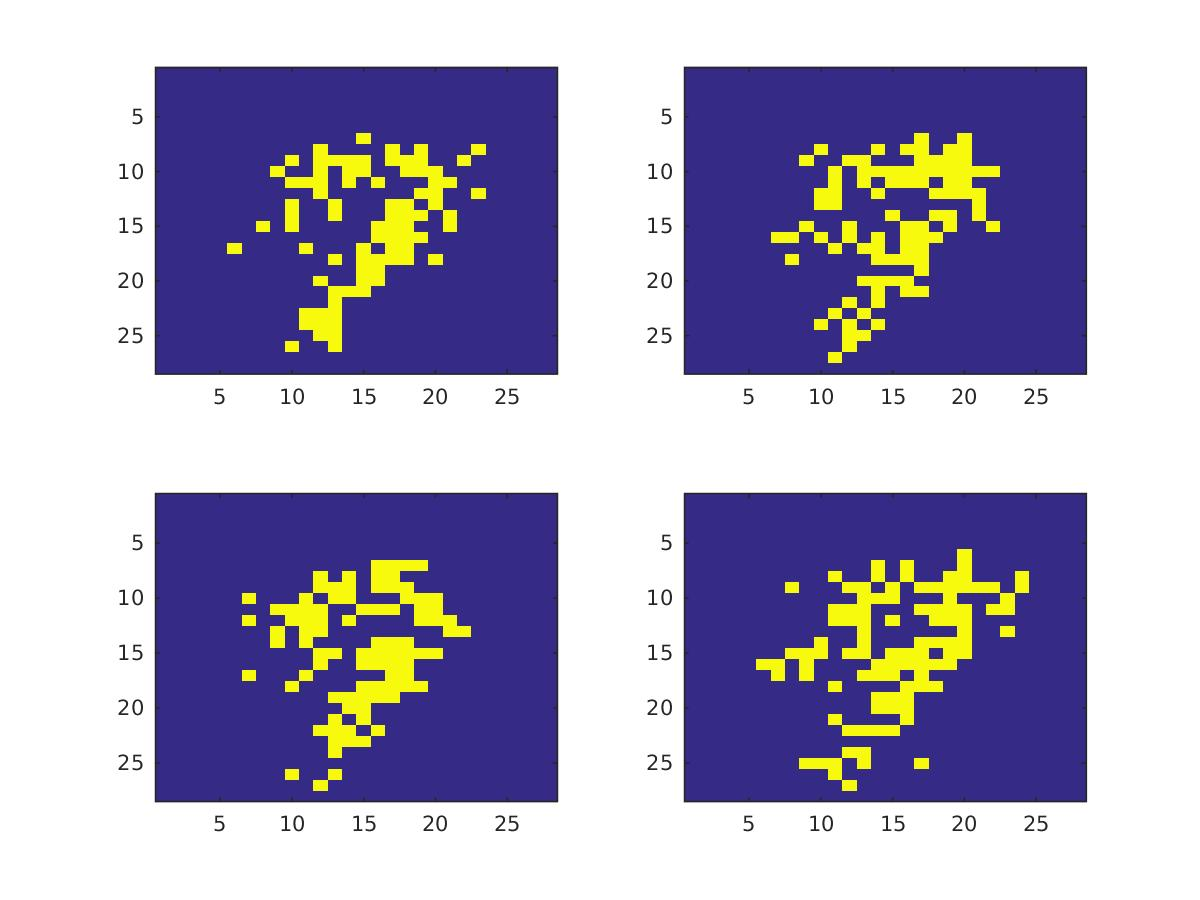
\includegraphics[scale=0.2]{samples}
\caption{Four Samples from the Bernoulli Model}
\end{figure}


Below it is shown a sample for each one of the 10 clusters.
\begin{figure}[H]
\centering
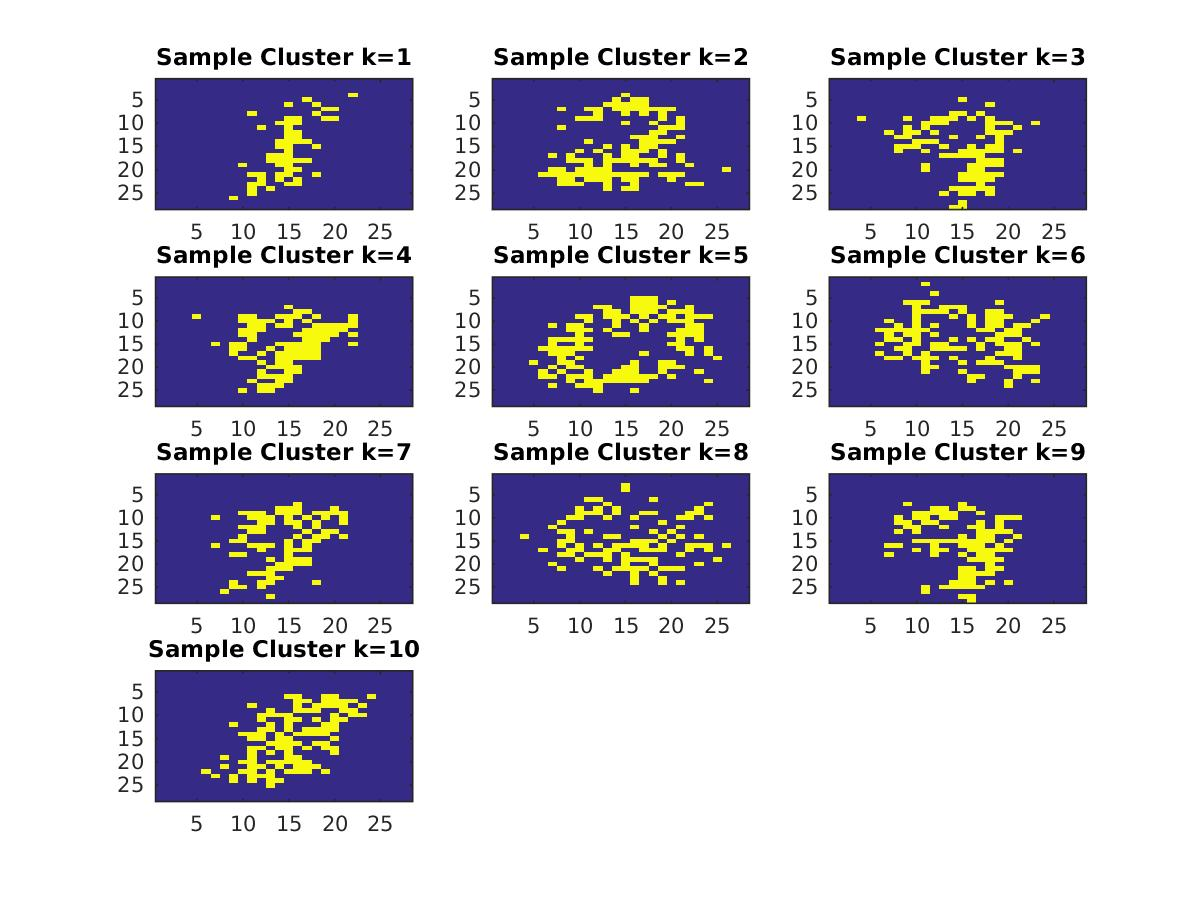
\includegraphics[scale=0.30]{cluster}
\caption{Samples for each of the ten clusters}
\end{figure} 

\newpage
\center{\section*{Project Proposal}}

%%%% Assignment Specific Stuff %%%%
\center{
\textbf{\title{Applications of Machine Learning to Stock Market Predictions}}
\newline
\author{Anson Wong, Gudbrand Duff Morris and Juan Garcia}
}
%\date{}

%\section{}
%\subsection{}
\flushleft
\section*{Introduction}

We propose to undertake an exploratory project on the potential impact of machine learning techniques to stock market prediction and analysis. 

The idea of using algorithms to predict the price of assets is as old as the stock exchange itself, and the existing body of work on the subject is huge. Therefore, \textbf
{the first part of our project will be an extensive literature review}. We will read and share interesting papers, using our findings to guide the development of the project scope and details.
\newline
Each one of the participants in this project have a possible idea in what direction this project could go:

\blu{Gudbrand's driving question:} With the dawn of the Era of Big Data upon us, I seek to discover if and how a "change in magnitude will produce a change in kind".

\blu{Anson's asks:} With the lack of insider information for amateur traders and the rise of algorithmic traders in the current stock market, is trading a lost cause for you and I? If not, then could an amateur machine learnist take a stab at trading and forecast price action with high success probability? I believe this is possible to earn large gains in nich\'{e} markets using a healthy amount of machine learning and understanding of human psychology. We plan to explore reinforcement learning and feature selection to achieve such a goal.

\blu{Juan's Idea:} A machine can perform better than a human in a wide range of situations. Forecasting and detecting patterns in the time series in the stock market could be one of these situations.
My idea is that with the techniques and ideas we are learning, we can teach a machine how to recognize what a good investment is. The criteria to define `good' comes from our knowledge 
from stock markets after doing some literature review. For the moment my first though in that direction is to apply the classification techniques we are learning,  in order to select the portfolio
with less variance. In this case the concept of `good' investment is `safe' investment.
\newline

Our literature research so far  is summarized below
\section*{Literature Review}


Papers: 
\begin{itemize}
\item http://www-stat.wharton.upenn.edu/~steele/Courses/434/434Context/EfficientMarket/AndyLoJPM2004.pdf

\item http://www-stat.wharton.upenn.edu/~steele/Courses/434/434Context/EfficientMarket/Granger-stockmarket.pdf

\end{itemize}

Interesting/useful links
\begin{itemize}
\item This guy is pretty great: \url{http://www-stat.wharton.upenn.edu/~steele/}
\item \url{https://www.udacity.com/course/machine-learning-for-trading--ud501}
\item \url{https://www.quantopian.com/posts/simple-machine-learning-example}
\item \url{http://www.qminitiative.org/UserFiles/files/S_Cl\%C3\%A9men\%C3\%A7on_ML.pdf}
\item \url{http://www-stat.wharton.upenn.edu/~steele/Courses/9xx/Resources/MLFinancialApplications/MLFinance.html}
\item \url{https://www.quora.com/How-do-financial-companies-use-machine-learning}
\item \url{http://techemergence.com/machine-learning-in-finance-applications/}
\item Our GoogleDrive: \url{https://drive.google.com/drive/folders/0B5_P6FZEZzQxOEN6ZTU1Q1czQTQ?usp=sharing}
\item R package for financial analysis: \url{https://cran.r-project.org/web/views/Finance.html}


\end{itemize}

\section*{Applications/Implementations/Ideas}

As the famous Oscar Wilde quote goes; "A cynic is a man who knows the price of everything but the value of nothing". In this sense, a ML model can be regarded as the ultimate cynic. The cynic has both advantages and disadvantages compared with the expert investor. With this in mind we have a set of potential topics/ideas to start with:

\begin{description}

\item[Predictability] How hard is the problem? Almost a philosophical question. 

\item[Clustering] What sort of stocks/bonds/instruments are there? Which models work for different categories?

\item[Feature Selection] Which features are important when it comes to prediction? We see many examples of seemingly godly predictions made based on the most complex features. Is this sort of 'thinking' possible for machines? Take for example the fictional Silicon Valley investor Peter Gregory, who reasons from the popularity of Burger King to the impending surge in periodic cicadas to Indonesian sesame futures. Or hedge fund manager Micheal Burry, one of the few big shot investors to recognize the subprime mortgage crisis long before it happened, just by analyzing the right data.

\item[Prediction techniques] How can we predict the behaviour of a stochastic PDE (Black Scholes')? 

\item[Momentum Investing] Gradient step based on today's winners. A potential winning strategy.

\item[Page Rank] Page rank is particularly useful for ranking connections (whether it be for search results, biological systems, social media influence). Although it might be a stretch, 
are there ways to use Page Rank to shed light on how the stock market works? 

\item[Q-learning] A method of reinforcement learning which sets up a reward system, and uses a mix of exploration and exploitation to achieve optimization of a goal. Planning to apply this to create a trading monkey.

\item[Financial Background] The introduction should get the reader up to date on the subject. Efficient markets, price, information, volatility, portfolio, ...

\item[Portfolio Selection] Real-time optimization++

\end{description}
Finally we consider some technical aspects regarding data sets and software.


\section*{Other}

\begin{itemize}

\item Datasets: There are plenty of sites were time series for the stock market can be accesed, such as, Finviz.com, Google Finance, Yahoo Finance, MarketWatch, to name a few. 

\item Programing Language and Packages: Any high level programing can be use to do the data analysis. At this point in the project there is some preference for $R$ 
and the financial analysis packages such as Empirical Finance. This is since there
is familiarity from the members of this research group with this language. 

\end{itemize}

\end{document} 



\end{document}
